\documentclass[12pt, a4paper]{article}

\usepackage[hmargin=2.5cm, vmargin=2cm]{geometry}
\usepackage{amsthm, amssymb, mathtools, yhmath, graphicx}
\usepackage{fontspec, type1cm, titlesec, titling, fancyhdr, tabularx}
\usepackage{color, unicode-math, float, hhline}

\usepackage[CheckSingle, CJKmath]{xeCJK}
\usepackage{CJKulem}
\usepackage{enumitem}
\usepackage{tikz}
\usepackage{circuitikz}
%\setCJKmainfont[BoldFont=cwTex Q Hei]{cwTex Q Ming}
%\setCJKsansfont[BoldFont=cwTex Q Hei]{cwTex Q Ming}
%\setCJKmonofont[BoldFont=cwTex Q Hei]{cwTex Q Ming}
\setCJKmainfont[BoldFont=cwTeX Q Hei]{cwTeX Q Ming}

\def\normalsize{\fontsize{12}{18}\selectfont}
\def\large{\fontsize{14}{21}\selectfont}
\def\Large{\fontsize{16}{24}\selectfont}
\def\LARGE{\fontsize{18}{27}\selectfont}
\def\huge{\fontsize{20}{30}\selectfont}

%\titleformat{\section}{\bf\Large}{\arabic{section}}{24pt}{}
%\titleformat{\subsection}{\large}{\arabic{subsection}.}{12pt}{}
%\titlespacing*{\subsection}{0pt}{0pt}{1.5ex}

\parindent=24pt

\DeclarePairedDelimiter{\abs}{\lvert}{\rvert}
\DeclarePairedDelimiter{\norm}{\lVert}{\rVert}
\DeclarePairedDelimiter{\inpd}{\langle}{\rangle}
\DeclarePairedDelimiter{\ceil}{\lceil}{\rceil}
\DeclarePairedDelimiter{\floor}{\lfloor}{\rfloor}

\newcommand{\img}{\mathsf{i}}
\newcommand{\ex}{\mathsf{e}}
\newcommand{\dD}{\mathrm{d}}
\newcommand{\dI}{\,\mathrm{d}}

\setenumerate{itemsep=0pt,topsep=0pt}

\title{EDA HW5}
\author{B02901178 江誠敏}
\begin{document}

\maketitle

\section{Problem 1.}
\begin{enumerate}
  \item No, since we don't know the exact amount of iteration $r$.
  \item Yes, as long as we know $W$ or $w_i$ is bounded (so that
    $W < n \max w_i$.
\end{enumerate}

\section{Problem 2.}
\begin{table}[H]
  \centering
\begin{tabular}{c|c|c|c|c|c|c}
  & swap & gain & $\Sigma$ gain & locked & $A$ & $B$ \\
  \hline
  1 & $(c, d)$ & $0$ & $0$ &$c, d$ & $a,b,d$ & $c, e, f$ \\
  \hline
  2 & $(b, f)$ & $-39$ & $-39$ & $b, c, d, f$ & $a,d,f$ & $c, b, e$ \\
  \hline
  3 & $(a, e)$ & $39$ & $0$ & $a,b,c,d,e,f$ & $d,e,f$ & $a, b, c$ \\
\end{tabular}
\end{table}

\section{Problem 3.}
We define
\begin{enumerate}
  \item Solution space: Each partition that split the vertice
    into to group with same size is in the solution space.
  \item Neighborhood structure: Let $(A, B)$ be a balanced
    partitioning. For all $a \in A, b \in B$, we swap these
    vertice and become a new partition $(A', B')$, then
    all these partition are the neighborhood of $(A, B)$.
  \item Cost Function: We define the total cost (cut size)
    to be our cost function.
\end{enumerate}
Then we could preform annealing. That is, set a random
initial state and temperature. Then each time, we
pick a random neighbor, calculate the cost difference,
and decide if we should go to the new state.

\section{Problem 4.}
First we compact the placement, and then derive the B-tree.
\begin{figure}[H]
  \centering
  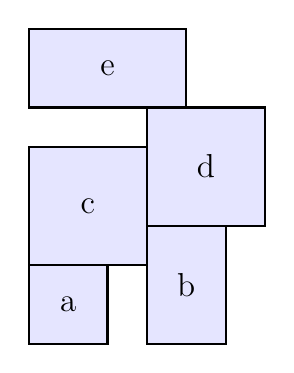
\begin{tikzpicture}[
    block/.style={fill=blue!10, thick},
    x=0.5cm,y=0.5cm
    ]
    \draw[block] (0, 0) rectangle (2, 2) node[pos=.5]{a};
    \draw[block] (0, 2) rectangle (3, 5) node[pos=.5]{c};
    \draw[block] (0, 6) rectangle (4, 8) node[pos=.5]{e};
    \draw[block] (3, 0) rectangle (5, 3) node[pos=.5]{b};
    \draw[block] (3, 3) rectangle (6, 6) node[pos=.5]{d};
  \end{tikzpicture}\hspace*{2cm}
  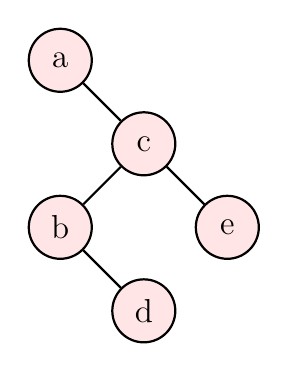
\begin{tikzpicture}[
    node/.style={circle,thick,draw,fill=red!10,minimum width=.8cm},
    x=1cm,y=1cm,node distance=1.5cm
    ]
    \node[node](a) at (0, 0){a};
    \node[node,below right of=a](c){c};
    \node[node,below right of=c](e){e};
    \node[node,below left of=c](b){b};
    \node[node,below right of=b](d){d};
    \draw[thick] (a) edge (c);
    \draw[thick] (c) edge (e);
    \draw[thick] (c) edge (b);
    \draw[thick] (b) edge (d);
  \end{tikzpicture}
\end{figure}

\begin{enumerate}
  \item (a): $[(0, 0), (0, 2), (2, 2), (2, 0)]$. 
  \item (c): $[(0, 0), (0, 5), (3, 5), (3, 0)]$. 
  \item (b): $[(0, 0), (0, 5), (3, 5), (3, 3), (5, 3), (5, 0)]$. 
  \item (d): $[(0, 0), (0, 5), (3, 5), (3, 6), (6, 6), (6, 0)]$. 
  \item (e): $[(0, 0), (0, 8), (4, 8), (4, 6), (6, 6), (6, 0)]$. 
\end{enumerate}
Area cost $= 48$.
Area efficiency $= 36/48 \approx 0.75\%$.

\section{Problem 5.}
\begin{figure}[H]
  \centering
  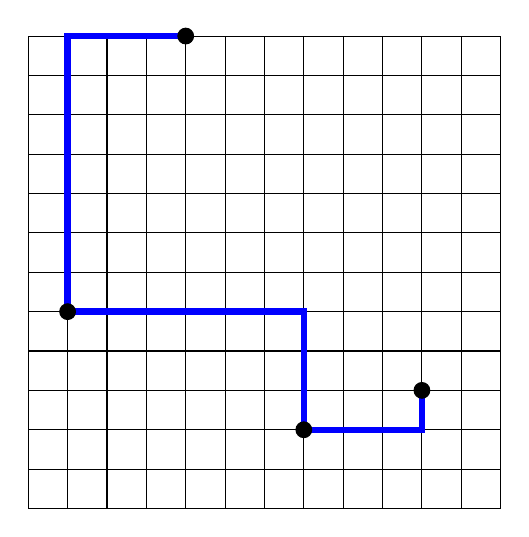
\begin{tikzpicture}[
    dot/.style={draw,circle,inner sep=2pt,fill},
    x=0.5cm,y=0.5cm,line/.style={line width=.8mm, blue}
    ]
    \draw[step=1] (0, 0) grid (12, 12);
    \draw[line] (10, 3) |- (7, 2) |- (1, 5) |- (4, 12);
    \node[dot] at (10, 3) {};
    \node[dot] at (4, 12) {};
    \node[dot] at (1, 5) {};
    \node[dot] at (7, 2) {};
  \end{tikzpicture}\hspace*{1.5cm}
  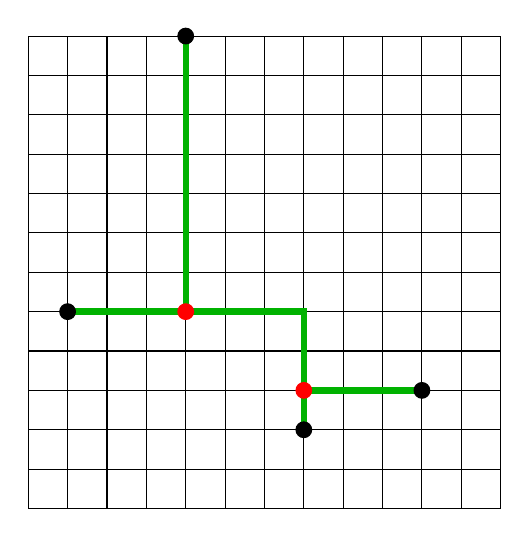
\begin{tikzpicture}[
    dot/.style={draw,circle,inner sep=2pt,fill},
    x=0.5cm,y=0.5cm,line/.style={line width=.8mm, green!70!black}
    ]
    \draw[step=1] (0, 0) grid (12, 12);
    \draw[line] (10, 3) -| (7, 2);
    \draw[line] (7, 2) |- (4, 5) -- (4, 12);
    \draw[line] (1, 5) -- (4, 5);
    \node[dot] at (10, 3) {};
    \node[dot] at (4, 12) {};
    \node[dot] at (1, 5) {};
    \node[dot] at (7, 2) {};
    \node[dot,red] at (4, 5) {};
    \node[dot,red] at (7, 3) {};
  \end{tikzpicture}\hspace*{2cm}
\end{figure}
\begin{align*}
  m &= 19 \\
  n &= 23 \\
  p &= 19 \\
  q &= 424 \\
  r &\approx 176.67 \\ 
  s &\approx 20.10 \\ 
\end{align*}

\section{Problem 6.}
\begin{enumerate}[label=(\alph*)]
  \item  $a = 10, b = 10, \text{err} = 0\%$.
  \item  $a = 10, b = 12, \text{err} = 16.7\%$.
  \item  $a = 10, b = 14, \text{err} = 28.6\%$.
  \item As the degree increase, the error rate increases. \\
    Using MST estimation or fit by some polynomial (i.e, 
    $\hat{b} = p a + q$, where $a$ is HPWL, $\hat{b}$ is 
    the new estimate, and $p, q$ are some parameter.) may
    give a better result.
\end{enumerate}


\section{Problem 7.}
We split a square into 4 nodes. That is, 
we use $(b, d)$ to represent a node, where $b$ is 
a square in the graph and $d$ is a direction,
which means that ``We traversed to the square $d$ with
the last direction facing $d$". Also we change the 
distance(cost) to a 2-tuple $(x, y)$ such that 
$x$ is the path length, and $y$ is the number of bends
on the path. We define
\[ (x_1, y_1) < (x_2, y_2) \quad \Leftrightarrow \quad 
  x_1 < x_2 \; \lor \; (x_1 = x_2 \; \land \; y_1 < y_2) \] 
and
\[ (x_1, y_1) + (x_2, y_2) = (x_1 + x_2, y_1 + y_2). \]
The distance from $(b_1, d_1)$ to $(b_2, d_2)$ is set to
$(1, 0)$ if $d_1 = d_2$ and $(1, 1)$ if $d_1 \neq d_2$, 
when $b_1, b_2$ are adjacent. Now set the distance 
$d(S, i) = 0$ for each of the $4$ distance and find 
the minimum path to $d(T, i)$ using any shortest
path finding algorithm gives the answer.

\section{Problem 8.}

\begin{figure}[H]
  \centering
  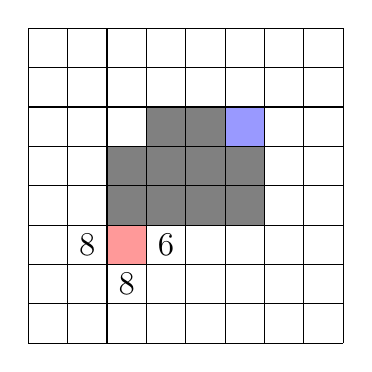
\begin{tikzpicture}[
    x=0.5cm,y=0.5cm
    ]
    \fill[gray] (2, 3) rectangle (6, 5);
    \fill[gray] (3, 5) rectangle (5, 6);
    \fill[blue!40] (5, 5) rectangle (6, 6);
    \fill[red!40] (2, 2) rectangle (3, 3);
    \draw[step=1] (0, 0) grid (8, 8);
    \node at (3.5, 2.5) {6};
    \node at (2.5, 1.5) {8};
    \node at (1.5, 2.5) {8};
  \end{tikzpicture}\hspace*{0.2cm}
  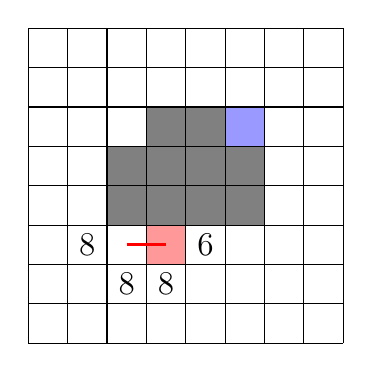
\begin{tikzpicture}[
    x=0.5cm,y=0.5cm,line/.style={very thick, red}
    ]
    \fill[gray] (2, 3) rectangle (6, 5);
    \fill[gray] (3, 5) rectangle (5, 6);
    \fill[blue!40] (5, 5) rectangle (6, 6);
    \fill[red!40] (3, 2) rectangle (4, 3);
    \draw[step=1] (0, 0) grid (8, 8);
    \node at (4.5, 2.5) {6};
    \node at (2.5, 1.5) {8};
    \node at (3.5, 1.5) {8};
    \node at (1.5, 2.5) {8};
    \draw[line] (2.5, 2.5) -- (3.5, 2.5);
  \end{tikzpicture}\hspace*{0.2cm}
  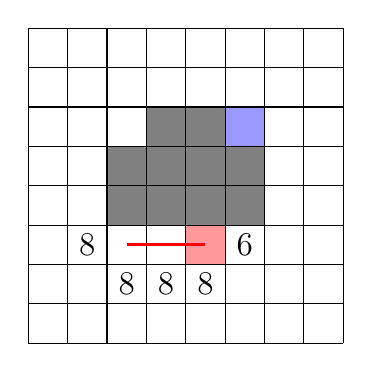
\begin{tikzpicture}[
    x=0.5cm,y=0.5cm,line/.style={very thick, red}
    ]
    \fill[gray] (2, 3) rectangle (6, 5);
    \fill[gray] (3, 5) rectangle (5, 6);
    \fill[blue!40] (5, 5) rectangle (6, 6);
    \fill[red!40] (4, 2) rectangle (5, 3);
    \draw[step=1] (0, 0) grid (8, 8);
    \node at (5.5, 2.5) {6};
    \node at (2.5, 1.5) {8};
    \node at (3.5, 1.5) {8};
    \node at (4.5, 1.5) {8};
    \node at (1.5, 2.5) {8};
    \draw[line] (2.5, 2.5) -- (4.5, 2.5);
  \end{tikzpicture}
  \vspace*{.5cm}

  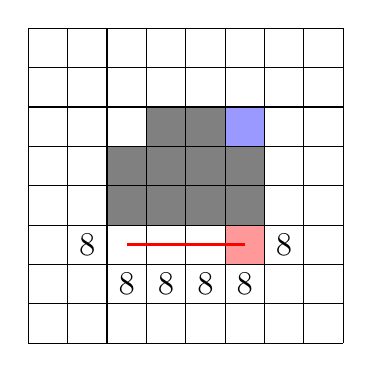
\begin{tikzpicture}[
    x=0.5cm,y=0.5cm,line/.style={very thick, red}
    ]
    \fill[gray] (2, 3) rectangle (6, 5);
    \fill[gray] (3, 5) rectangle (5, 6);
    \fill[blue!40] (5, 5) rectangle (6, 6);
    \fill[red!40] (5, 2) rectangle (6, 3);
    \draw[step=1] (0, 0) grid (8, 8);
    \node at (6.5, 2.5) {8};
    \node at (2.5, 1.5) {8};
    \node at (3.5, 1.5) {8};
    \node at (4.5, 1.5) {8};
    \node at (5.5, 1.5) {8};
    \node at (1.5, 2.5) {8};
    \draw[line] (2.5, 2.5) -- (5.5, 2.5);
  \end{tikzpicture}
  \hspace*{0.2cm}
  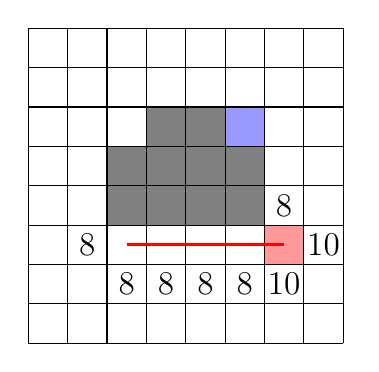
\begin{tikzpicture}[
    x=0.5cm,y=0.5cm,line/.style={very thick, red}
    ]
    \fill[gray] (2, 3) rectangle (6, 5);
    \fill[gray] (3, 5) rectangle (5, 6);
    \fill[blue!40] (5, 5) rectangle (6, 6);
    \fill[red!40] (6, 2) rectangle (7, 3);
    \draw[step=1] (0, 0) grid (8, 8);
    \node at (2.5, 1.5) {8};
    \node at (3.5, 1.5) {8};
    \node at (4.5, 1.5) {8};
    \node at (5.5, 1.5) {8};
    \node at (6.5, 1.5) {10};
    \node at (7.5, 2.5) {10};
    \node at (6.5, 3.5) {8};
    \node at (1.5, 2.5) {8};
    \draw[line] (2.5, 2.5) -- (6.5, 2.5);
  \end{tikzpicture}
  \hspace*{0.2cm}
  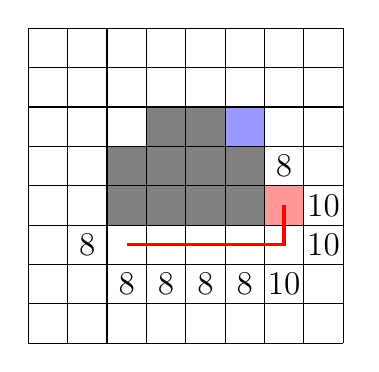
\begin{tikzpicture}[
    x=0.5cm,y=0.5cm,line/.style={very thick, red}
    ]
    \fill[gray] (2, 3) rectangle (6, 5);
    \fill[gray] (3, 5) rectangle (5, 6);
    \fill[blue!40] (5, 5) rectangle (6, 6);
    \fill[red!40] (6, 3) rectangle (7, 4);
    \draw[step=1] (0, 0) grid (8, 8);
    \node at (2.5, 1.5) {8};
    \node at (3.5, 1.5) {8};
    \node at (4.5, 1.5) {8};
    \node at (5.5, 1.5) {8};
    \node at (6.5, 1.5) {10};
    \node at (7.5, 2.5) {10};
    \node at (7.5, 3.5) {10};
    \node at (6.5, 4.5) {8};
    \node at (1.5, 2.5) {8};
    \draw[line] (2.5, 2.5) -| (6.5, 3.5);
  \end{tikzpicture}

  \vspace*{0.5cm}
  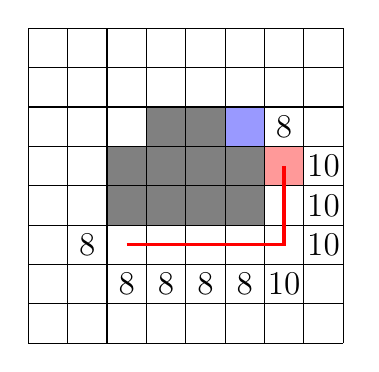
\begin{tikzpicture}[
    x=0.5cm,y=0.5cm,line/.style={very thick, red}
    ]
    \fill[gray] (2, 3) rectangle (6, 5);
    \fill[gray] (3, 5) rectangle (5, 6);
    \fill[blue!40] (5, 5) rectangle (6, 6);
    \fill[red!40] (6, 4) rectangle (7, 5);
    \draw[step=1] (0, 0) grid (8, 8);
    \node at (2.5, 1.5) {8};
    \node at (3.5, 1.5) {8};
    \node at (4.5, 1.5) {8};
    \node at (5.5, 1.5) {8};
    \node at (6.5, 1.5) {10};
    \node at (7.5, 2.5) {10};
    \node at (7.5, 3.5) {10};
    \node at (7.5, 4.5) {10};
    \node at (6.5, 5.5) {8};
    \node at (1.5, 2.5) {8};
    \draw[line] (2.5, 2.5) -| (6.5, 4.5);
  \end{tikzpicture}
  \hspace*{0.2cm}
  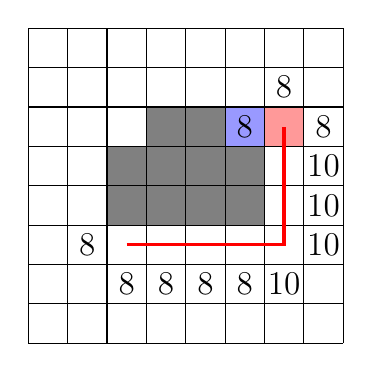
\begin{tikzpicture}[
    x=0.5cm,y=0.5cm,line/.style={very thick, red}
    ]
    \fill[gray] (2, 3) rectangle (6, 5);
    \fill[gray] (3, 5) rectangle (5, 6);
    \fill[blue!40] (5, 5) rectangle (6, 6);
    \fill[red!40] (6, 5) rectangle (7, 6);
    \draw[step=1] (0, 0) grid (8, 8);
    \node at (2.5, 1.5) {8};
    \node at (3.5, 1.5) {8};
    \node at (4.5, 1.5) {8};
    \node at (5.5, 1.5) {8};
    \node at (6.5, 1.5) {10};
    \node at (7.5, 2.5) {10};
    \node at (7.5, 3.5) {10};
    \node at (7.5, 4.5) {10};
    \node at (7.5, 5.5) {8};
    \node at (6.5, 6.5) {8};
    \node at (5.5, 5.5) {8};
    \node at (1.5, 2.5) {8};
    \draw[line] (2.5, 2.5) -| (6.5, 5.5);
  \end{tikzpicture}
  \hspace*{0.2cm}
  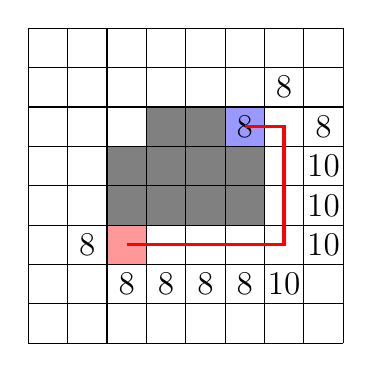
\begin{tikzpicture}[
    x=0.5cm,y=0.5cm,line/.style={very thick, red}
    ]
    \fill[gray] (2, 3) rectangle (6, 5);
    \fill[gray] (3, 5) rectangle (5, 6);
    \fill[blue!40] (5, 5) rectangle (6, 6);
    \fill[red!40] (2, 2) rectangle (3, 3);
    \draw[step=1] (0, 0) grid (8, 8);
    \node at (2.5, 1.5) {8};
    \node at (3.5, 1.5) {8};
    \node at (4.5, 1.5) {8};
    \node at (5.5, 1.5) {8};
    \node at (6.5, 1.5) {10};
    \node at (7.5, 2.5) {10};
    \node at (7.5, 3.5) {10};
    \node at (7.5, 4.5) {10};
    \node at (7.5, 5.5) {8};
    \node at (6.5, 6.5) {8};
    \node at (5.5, 5.5) {8};
    \node at (1.5, 2.5) {8};
    \draw[line] (2.5, 2.5) -| (6.5, 5.5) -- ++(-1, 0);
  \end{tikzpicture}
\end{figure}

\section{Problem 9.}

\begin{figure}[H]
  \centering
  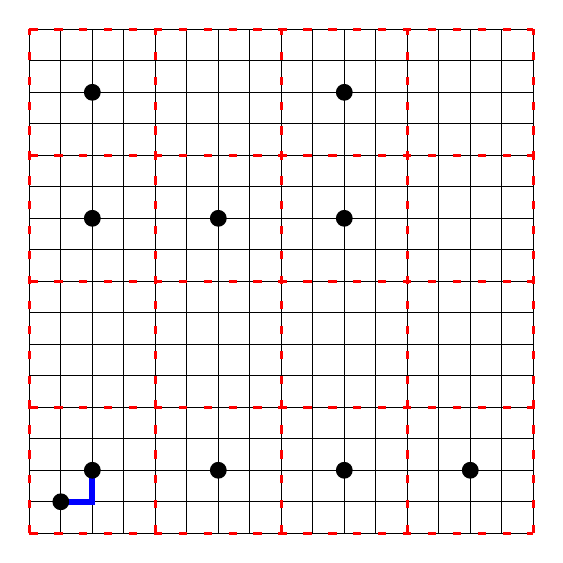
\begin{tikzpicture}[
    x=0.4cm,y=0.4cm,dot/.style={draw,black,fill,circle,inner sep=2pt}
    ]
    \draw[step=1] (0, 0) grid (16, 16);
    \draw[step=4,very thick,red,loosely dashed] (0, 0) grid (16, 16);
    \draw[blue, line width=.8mm] (1, 1) -| (2, 2);
    \node[dot] at (1, 1) {};
    \node[dot] at (2, 2) {};
    \node[dot] at (2, 10) {};
    \node[dot] at (2, 14) {};
    \node[dot] at (6, 2) {};
    \node[dot] at (10, 10) {};
    \node[dot] at (6, 10) {};
    \node[dot] at (10, 14) {};
    \node[dot] at (10, 2) {};
    \node[dot] at (14, 2) {};
  \end{tikzpicture}\hspace*{0.2cm}
  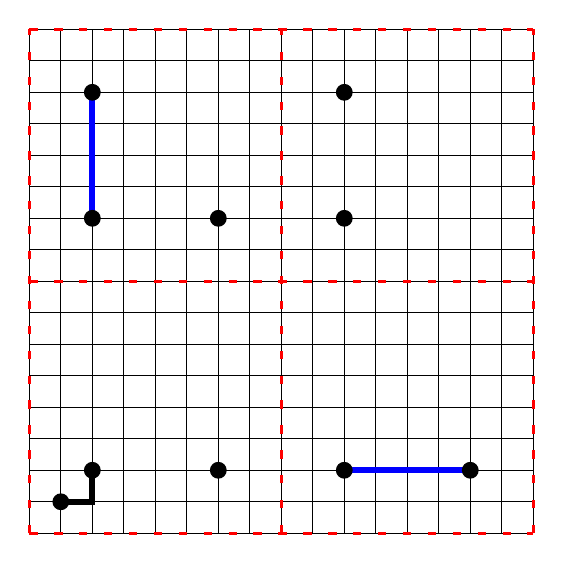
\begin{tikzpicture}[
    x=0.4cm,y=0.4cm,dot/.style={draw,black,fill,circle,inner sep=2pt}
    ]
    \draw[step=1] (0, 0) grid (16, 16);
    \draw[step=8,very thick,red,loosely dashed] (0, 0) grid (16, 16);
    \draw[black, line width=.8mm] (1, 1) -| (2, 2);
    \draw[blue, line width=.8mm] (2, 10) -| (2, 14);
    \draw[blue, line width=.8mm] (10, 2) -| (14, 2);
    \node[dot] at (1, 1) {};
    \node[dot] at (2, 2) {};
    \node[dot] at (2, 10) {};
    \node[dot] at (2, 14) {};
    \node[dot] at (6, 2) {};
    \node[dot] at (10, 10) {};
    \node[dot] at (6, 10) {};
    \node[dot] at (10, 14) {};
    \node[dot] at (10, 2) {};
    \node[dot] at (14, 2) {};
  \end{tikzpicture}

  \vspace{.5cm}
  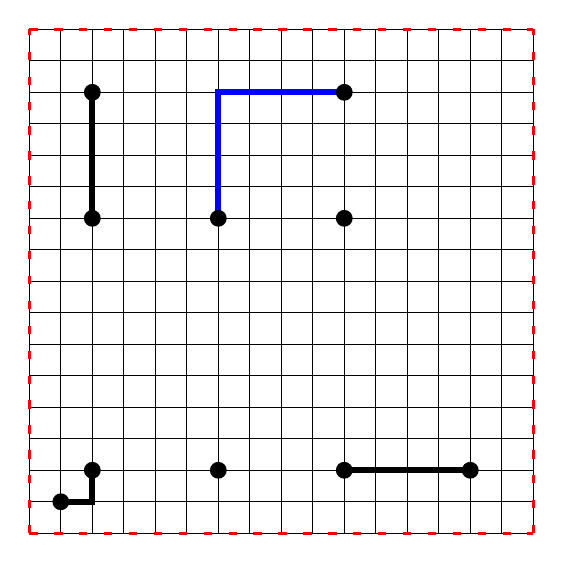
\begin{tikzpicture}[
    x=0.4cm,y=0.4cm,dot/.style={draw,black,fill,circle,inner sep=2pt}
    ]
    \draw[step=1] (0, 0) grid (16, 16);
    \draw[step=16,very thick,red,loosely dashed] (0, 0) grid (16, 16);
    \draw[black, line width=.8mm] (1, 1) -| (2, 2);
    \draw[black, line width=.8mm] (2, 10) -| (2, 14);
    \draw[black, line width=.8mm] (10, 2) -| (14, 2);
    \draw[blue, line width=.8mm] (6, 10) |- (10, 14);
    \node[dot] at (1, 1) {};
    \node[dot] at (2, 2) {};
    \node[dot] at (2, 10) {};
    \node[dot] at (2, 14) {};
    \node[dot] at (6, 2) {};
    \node[dot] at (10, 10) {};
    \node[dot] at (6, 10) {};
    \node[dot] at (10, 14) {};
    \node[dot] at (10, 2) {};
    \node[dot] at (14, 2) {};
  \end{tikzpicture}\hspace*{0.2cm}
  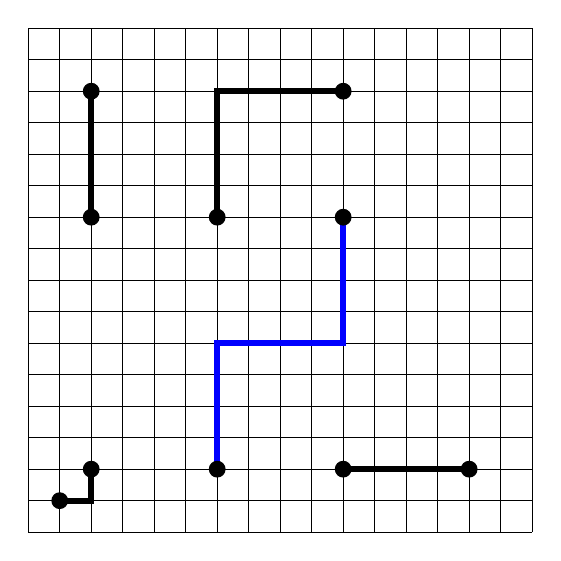
\begin{tikzpicture}[
    x=0.4cm,y=0.4cm,dot/.style={draw,black,fill,circle,inner sep=2pt}
    ]
    \draw[step=1] (0, 0) grid (16, 16);
    \draw[black, line width=.8mm] (1, 1) -| (2, 2);
    \draw[black, line width=.8mm] (2, 10) -| (2, 14);
    \draw[black, line width=.8mm] (10, 2) -| (14, 2);
    \draw[black, line width=.8mm] (6, 10) |- (10, 14);
    \draw[blue, line width=.8mm] (6, 2) |- (8, 6) -| (10, 10);
    \node[dot] at (1, 1) {};
    \node[dot] at (2, 2) {};
    \node[dot] at (2, 10) {};
    \node[dot] at (2, 14) {};
    \node[dot] at (6, 2) {};
    \node[dot] at (10, 10) {};
    \node[dot] at (6, 10) {};
    \node[dot] at (10, 14) {};
    \node[dot] at (10, 2) {};
    \node[dot] at (14, 2) {};
  \end{tikzpicture}
\end{figure}

\end{document}

